\documentclass{beamer}

\usepackage{tikz}
\usetikzlibrary{positioning,matrix, arrows.meta}
\usetikzlibrary{graphdrawing.trees}
\usepackage{color}
\newcommand{\vet}[1]{\foreach \num in {#1}{\el{\num}}}
\newcommand{\vetempty}[1]{\foreach \num in {#1}{\elempty{\num}}}
\newcommand{\el}[1]{\tikz{\node[font=\smaller, draw]{#1}}}
\newcommand{\elempty}[1]{\tikz{\node[font=\small, minimum size=1cm, draw=white, fill=white]{#1}}}
\newcommand{\bl}{\color{blue}}
\newcommand{\gr}{\color{gray}}
\newcommand{\re}{\color{red}}
\newcommand{\tcb}[1]{\textcolor{blue}{#1}}
\newcommand{\tcg}[1]{\textcolor{green}{#1}}
\newcommand{\tcr}[1]{\textcolor{red}{#1}}
\newcommand{\ar}{\tikz{\draw [->] (0,0) -- (0,0.4)}}
\newcommand{\nd}{\color{white!0}.}

\usepackage{beamerthemeSingapore}
\usepackage{graphicx}
%\usepackage{here}
\usepackage{url}
\usepackage[brazil]{babel}
\usepackage[T1]{fontenc}
\usepackage[utf8]{inputenc}
%\usepackage[tight,raggedright]{subfigure}
\usepackage{subfigure}
\usepackage[alf]{abntex2cite}
\usepackage{listings}
\usepackage{minted}
\usepackage{algorithm2e}
\usepackage{amsmath}
\usepackage{pdfpages}
% Please add the following required packages to your document preamble:
\usepackage{booktabs}
\usepackage{ragged2e}
\usepackage{etoolbox}
\usepackage{mathtools}
\usepackage{caption}
\usepackage{xmpmulti}

\tikzset{
  treenode/.style = {align=center, inner sep=0pt, text centered,
    font=\sffamily},
  arn_b/.style = {treenode, circle, black, font=\sffamily\bfseries, draw=black,
    fill=white, text width=1.5em},% arbre rouge noir, noeud noir
  arn_n/.style = {treenode, circle, white, font=\sffamily\bfseries, draw=black,
    fill=black, text width=1.5em},% arbre rouge noir, noeud noir
  arn_r/.style = {treenode, circle, red, draw=red, 
    text width=1.5em, very thick},% arbre rouge noir, noeud rouge
  arn_x/.style = {treenode, rectangle, draw=black,
    minimum width=0.5em, minimum height=0.5em}% arbre rouge noir, nil
}

\captionsetup[figure]{labelformat=empty,textfont=smaller}

\DeclarePairedDelimiter{\ceil}{\lceil}{\rceil}

\apptocmd{\frame}{}{\justifying}{} % Allow optional arguments after frame.

% TODO TODO TODO TODO TODO TODO TODO
\title{07 - Árvores}
\author{Prof. Alex Kutzke}
\date{Junho de 2021}

\begin{document}

% ==========================================
\begin{frame}
  \begin{center}
    % TODO TODO TODO TODO TODO TODO
    \large{Setor de Educação Profissional e Tecnológica}\\
    Tecnologia em Análise e Desenvolvimento de Sistemas\\
    \vspace{1cm}			
    \small{DS141 - Estruturas de Dados II}
  \end{center}
  \titlepage

  \begin{center}
    Slides adaptados do material produzido\\pelo Prof. Rodrigo Minetto
  \end{center}
\end{frame}
% ==========================================

% ==========================================
\begin{frame}[c]{Roteiro}
  \tableofcontents

\end{frame}
% ==========================================

\section{Motivação e conceito}

\begin{frame}[c]{Motivação}
  Examinamos até agora estruturas de dados que podem ser
  chamadas de lineares, como vetores e listas. A importância dessas estruturas 
  é inegável, mas: 
  \begin{itemize}
    \item Elas não são adequadas para representar dados que devem ser dispostos de maneira \tcb{hierárquica};
    \item É necessário buscar estruturas \tcb{mais eficientes} para a implementação de tabelas de símbolos (inserção, atualização, busca e remoção).
  \end{itemize}
\end{frame}

\begin{frame}
  \frametitle{Exemplo de Representação Hierárquica}

  \textbf{Sistema de arquivos}: arquivos e diretórios dentro de diretórios, ...;

  \begin{figure}
    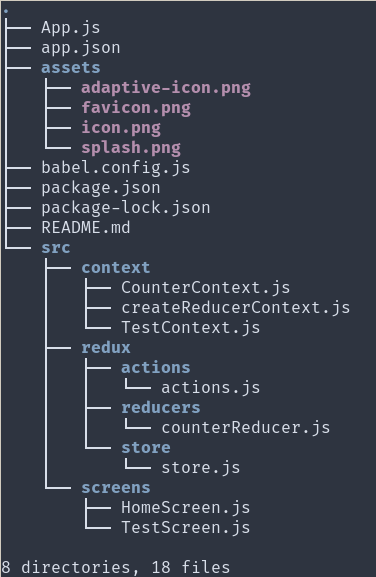
\includegraphics[width=.4\textwidth]{img/tree.png}
  \end{figure}
\end{frame}

\begin{frame}
  \frametitle{Árvores}

  \begin{itemize}
    \item No contexto da computação são \tcr{estuturas de dados} não sequenciais que seguem o conceito
          de \tcb{hierarquia}. 
    \item A forma mais natural de definir uma estrutura de árvore é usando a 
          \tcr{recursividade}.
  \end{itemize}
\end{frame}

\begin{frame}
  \frametitle{Definição}

  Uma árvore é um conjunto finito de \tcr{n} estruturas elementares chamados \tcb{nós}.
  Tal que se $n > 0$, então:

  \begin{itemize}
    \item existe um nó especial \tcr{r}, denominado \tcb{raiz} da árvore;
    \item os nós restantes sâo particionados em $m$ conjuntos disjuntos (chamado de
          \tcb{subárvores} de \tcr{r}), tal que, cada um desses conjuntos é também
          uma árvore.
  \end{itemize}
\end{frame}

\begin{frame}[t]
  \frametitle{Árvores}

  Na computação: 
  \begin{itemize}
    \item<1-> as árvores são representadas de baixo para cima;
    \item<2-> da raiz às folhas;
    \item<3-> cada bifurcação é um nó interno. Cada folha é um nó externo.
  \end{itemize}

  \begin{figure}[h]
    \centering
    \only<1>{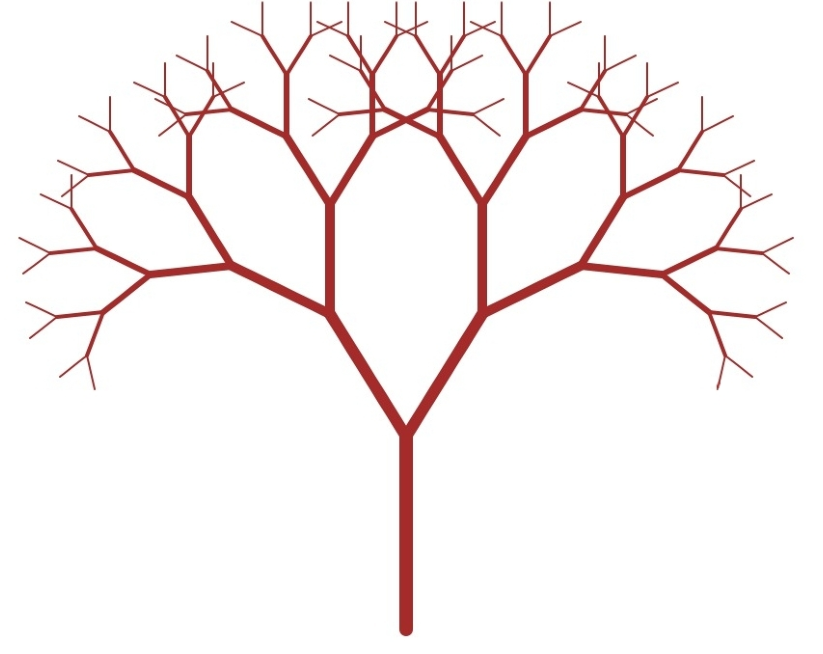
\includegraphics[width=.5\textwidth]{img/pseudo_tree.png}}
    \only<2>{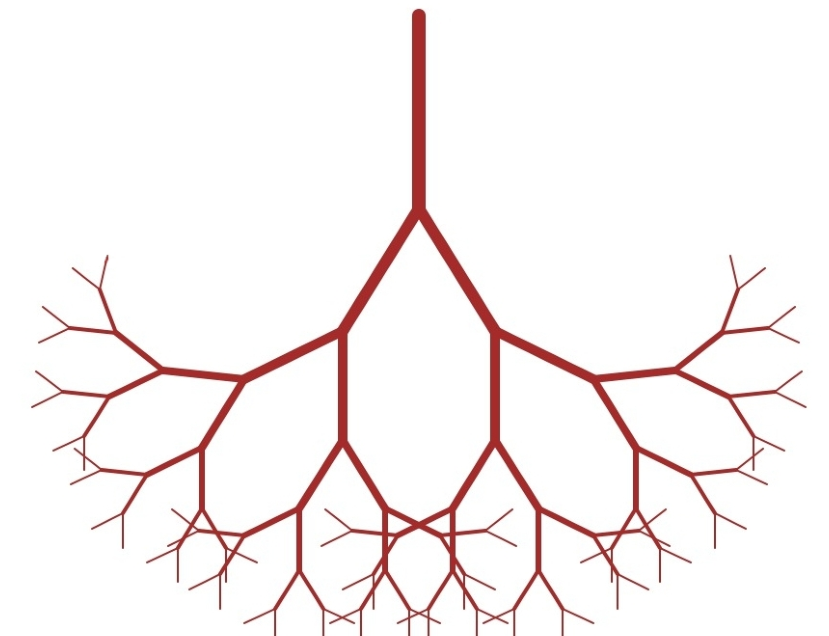
\includegraphics[width=.5\textwidth]{img/pseudo_tree2.png}}
    \only<3>{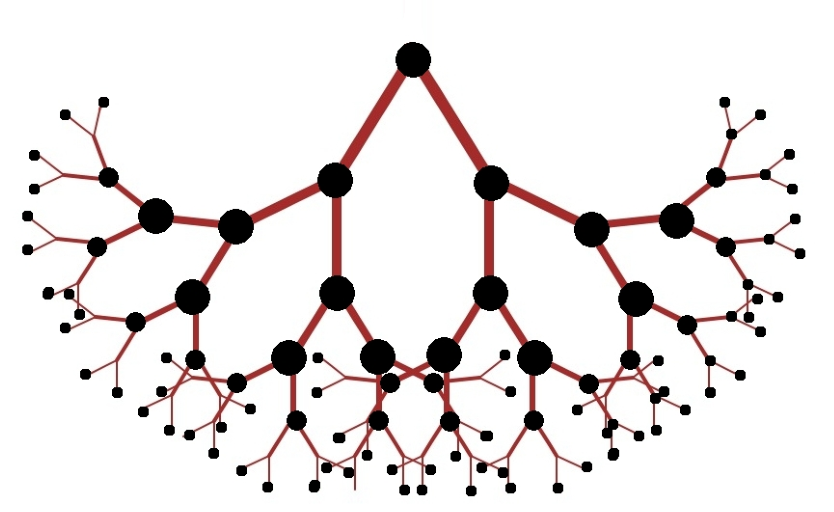
\includegraphics[width=.5\textwidth]{img/pseudo_tree3.png}}
  \end{figure}
\end{frame}

\begin{frame}
  \frametitle{Árvores}
  Ao adotar essa forma de representação, não é necessário representar
  explicitamente a \tcr{direção dos ponteiros} (do ``galhos'').
  
  \begin{figure}[h]
    \centering
    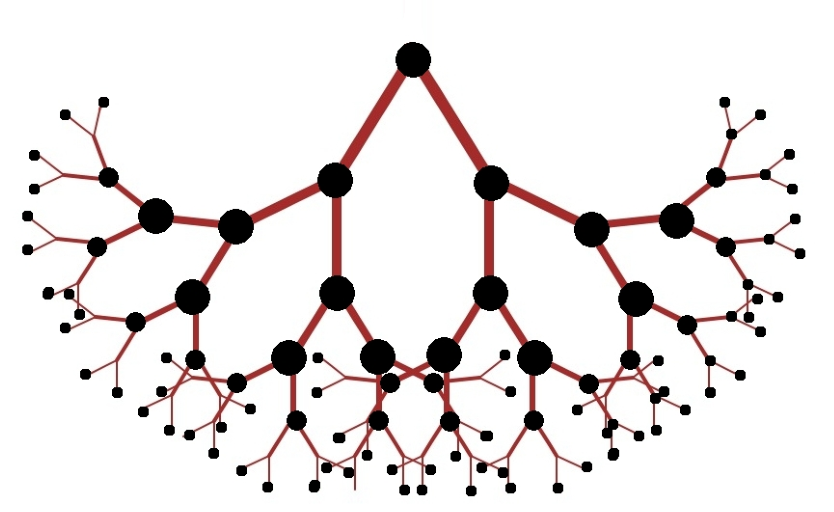
\includegraphics[width=.5\textwidth]{img/pseudo_tree3.png}
  \end{figure}

  \textbf{Apontam sempre do pai para os filhos}.
\end{frame}

\begin{frame}
  \frametitle{Conceitos}

  \begin{description}
    \item[Grau de um nó] número de subárvores de um nó;
    \item[Grau da árvore] grau máximo entre todos os nós;
    \item[Nó folha] nó com grau 0 (sem subárvores).
  \end{description}

  \begin{itemize}
    \item O nó raiz tem um \textbf{nível} 0, filhos do nó raiz tem nível 1 e,
          assim, sucessivamente;
    \item \textbf{Árvores binárias} são árvores cujos nós tem grau 0, 1 ou 2 (ou seja,
          tem no máximo 2 filhos);
    \item Um conjunto de árvores disjuntas forma uma floresta;
    \item Nós com filhos são chamados de \textbf{nós internos};
    \item Nós sem filhos são chamados de \textbf{nós externos}.
  \end{itemize}
\end{frame}

\section{Árvores binárias}

\begin{frame}[c]
  \frametitle{Árvore binária}

  \begin{itemize}
    \item Uma subárvore de uma árvore binária é sempre especificada como sendo
          a subárvore da \tcb{esquerda} ou da \tcb{direita};
    \item Qualquer uma das subárvores pode ser vazia;
  \end{itemize}

  \vspace{0.5cm}

  \begin{columns}
    \begin{column}{0.3\textwidth}
      \centering
      \begin{tikzpicture}[nodes={draw, circle},-]
        \node{a}
        child { node {b} }
        child { node {c} };
      \end{tikzpicture}
    \end{column}
    \begin{column}{0.3\textwidth}
      \centering
      \begin{tikzpicture}[nodes={draw, circle},-]
        \node{a}
        child { node {b} }
        child [ missing ];
      \end{tikzpicture}
    \end{column}
    \begin{column}{0.3\textwidth}
      \centering
      \begin{tikzpicture}[nodes={draw, circle},-]
        \node{a}
        child [ missing ]
        child { node {c} };
      \end{tikzpicture}
    \end{column}
  \end{columns}
\end{frame}

\begin{frame}[fragile,t]
  \frametitle{Estrutura}

  \begin{columns}
    \begin{column}{0.4\textwidth}
      \begin{minted}[frame=lines,framesep=2mm,baselinestretch=1,fontsize=\normalsize,linenos]{c}
typedef struct arvore {
  char info;
  struct arvore *esq;
  struct arvore *dir;
} Arvore;
      \end{minted}
    \end{column}
    \begin{column}{0.4\textwidth}
      \centering
      \begin{tikzpicture}[-]
        \node at (0,-1) (root) [arn_b] {a}
        child { node [arn_b] {b} edge from parent node [above,left] {*esq} }
        child { node [arn_b] {c} edge from parent node [above,right] {*dir} };
        \only<2>{\draw [->] (0,0) node [above] {Raiz} -- (root) ;}
      \end{tikzpicture}
    \end{column}
  \end{columns}
  
  \vspace{1cm}
  \only<2>{
    \begin{itemize}
      \item Podemos representar a árvore com apenas um ponteiro para seu elemento raiz;
    \end{itemize}
  }

\end{frame}

\section{Operações básicas}

\begin{frame}[fragile]
  \frametitle{Operações}

  \begin{itemize}
    \item Como todo \textbf{tipo abstrato de dados (TAD)}, a estrutura de dado deve vir acompanhada de \tcb{operações};
    \item As operações dependem do uso que se pretende do TAD;
    \item Um conjunto de operações possíveis para um TAD de árvore binária poderia ser:
  \end{itemize}

  \begin{minted}[frame=lines,framesep=2mm,baselinestretch=1,fontsize=\normalsize,linenos]{c}
// arquivo arvore.h
Arvore* cria_arv_vazia (void);
Arvore* arv_constroi (char c, Arvore* e, Arvore* d);
Arvore* arv_libera (Arvore* a);
int     verifica_arv_vazia (Arvore* a);
int     arv_pertence (Arvore* a, char c);
void    arv_imprime (Arvore* a);
  \end{minted}
\end{frame}

\begin{frame}[fragile]
  \frametitle{Operações - Criar árvore vazia}

  \begin{itemize}
    \item Como a árvore é representada pelo endereço do nó raiz, uma árvore \tcb{vazia} pode ser representada por um ponteiro nulo:
  \end{itemize}

  \begin{minted}[frame=lines,framesep=2mm,baselinestretch=1,fontsize=\normalsize,linenos]{c}
Arvore* cria_arv_vazia (void) {
  return NULL;
}
  \end{minted}
\end{frame}

\begin{frame}[fragile]
  \frametitle{Operações - Construir árvore}

  \begin{itemize}
    \item A construção de árvores não vazias pode ser realizada com 3 itens:
    \begin{enumerate}
      \item Item a ser armazenado no nó raiz;
      \item Ponteiro para subárvore da esquerda;
      \item Ponteiro para subárvore da direita;
    \end{enumerate}
  \end{itemize}

  \begin{minted}[frame=lines,framesep=2mm,baselinestretch=1,fontsize=\normalsize,linenos]{c}
Arvore* arv_constroi (char c, Arvore* e, Arvore* d) {
  Arvore* a = (Arvore*)malloc(sizeof(Arvore));
  a->info = c;
  a->esq = e;
  a->dir = d;
  return a;
}
  \end{minted}

  \visible<2>{
    É claro que uma função de inserir elemento na árvore, ao invés de criar uma árvore para um único elemento, é muito mais útil. Mas veremos isso em breve.
  }
\end{frame}

\begin{frame}[fragile]
  \frametitle{Operações - Verifica árvore vazia}

  \begin{itemize}
    \item Para verificar se uma árvore está vazia, basta um único teste:
  \end{itemize}

  \begin{minted}[frame=lines,framesep=2mm,baselinestretch=1,fontsize=\normalsize,linenos]{c}
int verifica_arv_vazia (Arvore* a) {
  return (a == NULL);
}
  \end{minted}
\end{frame}

\begin{frame}[fragile]
  \frametitle{Operações - Liberar}

  \begin{itemize}
    \item Para liberar o espaço alocado por uma árvore, precisamos liberar as subárvores também;
    \item Uma função recursiva pode resolver esse problema:
  \end{itemize}

  \begin{minted}[frame=lines,framesep=2mm,baselinestretch=1,fontsize=\normalsize,linenos]{c}
Arvore* arv_libera (Arvore* a) {
    if (!verifica_arv_vazia(a)) {
    arv_libera (a->esq);
    arv_libera (a->dir);
    free(a);
  }
    return NULL;
}
  \end{minted}
  
  \begin{itemize}
    \item A ordem das chamadas recursivas e do free importa! 
  \end{itemize}
\end{frame}

\begin{frame}[c]
  \frametitle{Exemplo: Contrução de árvore}

  \centering
  \begin{tikzpicture}[-]
    \node (root) [arn_b] {a}
    child { 
      node [arn_b] {b} 
      child [missing] 
      child { node [arn_b] {d} } 
    }
    child [missing] 
    child { 
      node [arn_b] {c} 
      child { node [arn_b] {e} } 
      child { node [arn_b] {f} } 
    };
  \end{tikzpicture}

\end{frame}

\begin{frame}[fragile]
  \frametitle{Exemplo: Contrução de árvore}

  \begin{minted}[frame=lines,framesep=2mm,baselinestretch=1,fontsize=\normalsize,linenos]{c}
int main (int argc, char *argv[]) {
  Arvore *a, *a1, *a2, *a3, *a4, *a5;
  a1 = arv_constroi('d',cria_arv_vazia(),cria_arv_vazia());
  a2 = arv_constroi('b',cria_arv_vazia(),a1);
  a3 = arv_constroi('e',cria_arv_vazia(),cria_arv_vazia());
  a4 = arv_constroi('f',cria_arv_vazia(),cria_arv_vazia());
  a5 = arv_constroi('c',a3,a4);
  a  = arv_constroi('a',a2,a5);
  return 0;
}
  \end{minted}
\end{frame}


\begin{frame}[fragile]
  \frametitle{Exemplo: Contrução de árvore}

  Alternativamente, podemos criar a árvore com uma \tcb{única atribuição}, seguindo uma
  \textbf{estrutura recursivamente}:

  \begin{minted}[frame=lines,framesep=2mm,baselinestretch=1,fontsize=\small,linenos]{c}
Arvore *a = arv_constroi ('a',
  arv_constroi('b',
    cria_arv_vazia(),
    arv_constroi('d',cria_arv_vazia(),cria_arv_vazia())
  ),
  arv_constroi('c',
    arv_constroi('e',cria_arv_vazia(),cria_arv_vazia()),
    arv_constroi('f',cria_arv_vazia(),cria_arv_vazia())
  )
);
  \end{minted}
\end{frame}

\begin{frame}[fragile]
  \frametitle{Contrução de árvore}

  \begin{itemize}
    \item Devemos notar que a definição de árvore, por ser recursiva, não faz distinção 
          entre árvores e subárvores;
    \item A função arv\_constroi pode ser usada para acrescentar (``enxertar'') uma subárvore 
          em um ramo de uma árvore.
  \end{itemize}

  \begin{minted}[frame=lines,framesep=2mm,baselinestretch=1,fontsize=\small,linenos]{c}
a->esq->esq = arv_constroi ('x',
arv_constroi('y',cria_arv_vazia(),cria_arv_vazia()),
arv_constroi('z',cria_arv_vazia(),cria_arv_vazia())
  \end{minted}
\end{frame}

\begin{frame}[c]
  \frametitle{Resultado}

  \centering
  \begin{tikzpicture}[-]
    \node (root) [arn_b] {a}
    child { 
      node [arn_b] {b} 
      child {
        node [arn_b] {x}
        child {node [arn_b] {y}}
        child {node [arn_b] {z}}
      }
      child [missing]
      child { node [arn_b] {d} } 
    }
    child [missing] 
    child [missing]
    child { 
      node [arn_b] {c} 
      child { node [arn_b] {e} } 
      child [missing]
      child { node [arn_b] {f} } 
    };
  \end{tikzpicture}

\end{frame}

\section{Exercícios propostos}

\begin{frame}
  \frametitle{Exercícios propostos}

  \textbf{Exercício 1} Escreva uma função que recebe uma árvore binária
  com entrada e imprime seus nós. Por exemplo, supondo como
  entrada a árvore abaixo, a impressão desejada é representada por:
  \texttt{a b d c e f}

  \centering
  \begin{tikzpicture}[-]
    \node (root) [arn_b] {a}
    child { 
      node [arn_b] {b} 
      child [missing]
      child { node [arn_b] {d} } 
    }
    child [missing]
    child { 
      node [arn_b] {c} 
      child { node [arn_b] {e} } 
      child { node [arn_b] {f} } 
    };
  \end{tikzpicture}

\end{frame}

\begin{frame}
  \frametitle{Exercícios propostos}

    \textbf{Exercício 2} Para descrever árvores binárias, podemos usar a seguinte notação textual: 
    a árvore vazia é representada por \texttt{<>}, e árvores não-vazias, por 
    \texttt{< raiz esq dir >}. Com essa notação, a árvore abaixo é representada por:\\
    \texttt{<a <b <> <d <> <> > ><c <e <><> ><f <> <> > > >}\\
    Escreva uma função que recebe uma árvore de entrada e a imprime nessa notação.

  \centering
  \begin{tikzpicture}[-]
    \node (root) [arn_b] {a}
    child { 
      node [arn_b] {b} 
      child [missing]
      child { node [arn_b] {d} } 
    }
    child [missing]
    child { 
      node [arn_b] {c} 
      child { node [arn_b] {e} } 
      child { node [arn_b] {f} } 
    };
  \end{tikzpicture}

\end{frame}

\begin{frame}[fragile]
  \frametitle{Exercícios propostos}

  \textbf{Exercício 3} Escreva uma função que retorna um valor booleano (um ou zero) que indica a 
  ocorrência ou não de um dado caractere na árvore. Considere o seguinte protótipo para
  a sua função:

  \begin{minted}[frame=lines,framesep=2mm,baselinestretch=1,fontsize=\small,linenos]{c}
int arv_pertence (Arvore *a, char c);
  \end{minted}

  onde \texttt{char c} é o caractere que deve ser procurado na árvore a.

\end{frame}

% ==========================================
% Frame para referências
\begin{frame}[allowframebreaks]
  \frametitle{Referências utilizadas na apresentação}
  \bibliography{referencias}
\end{frame}
% ==========================================

\end{document}
